% Metaboenrich: directed absorbing random walk on the metabolite-reaction network
% Compiles on Overleaf with pdfLaTeX (standard packages only).
\documentclass[11pt]{article}

\usepackage[margin=1in]{geometry}
\usepackage[T1]{fontenc}
\usepackage{lmodern}
\usepackage{amsmath,amssymb,amsthm}
\usepackage{booktabs}
\usepackage{tabularx}
\usepackage{enumitem}
\usepackage{xcolor}
\usepackage{tikz}
\usetikzlibrary{arrows.meta,positioning}
\usepackage[colorlinks=true,linkcolor=blue!50!black,urlcolor=blue!50!black,citecolor=blue!50!black]{hyperref}

\newcommand{\code}[1]{\texttt{#1}}
\newcommand{\R}{\mathbb{R}}
\newcommand{\Sset}{\mathcal{S}}
\newcommand{\Tset}{\mathcal{T}}
\newcommand{\X}{\mathcal{X}}
\newcommand{\fwd}{{\rightarrow}}
\newcommand{\bwd}{{\leftarrow}}
\newtheorem*{remark}{Remark}
\newtheorem*{proposition}{Proposition}

\title{Metaboenrich step 5 (experimental):\\
a directed absorbing random walk conditioned on absorption}
\author{Metaboenrich methods note}
\date{Code reference: \code{metaboenrich/walk.py}, commit \code{0f6c135} (branch \code{directed-rw}); option \code{--mode walk}}

\begin{document}
\maketitle

\begin{abstract}
The default Metaboenrich scoring step, Ohm's-law current flow, solves an electrical
problem on the \emph{undirected} metabolite--reaction graph. It ignores reaction
directions and lets current pass between two substrates of the same reaction. This
note describes the experimental alternative. Walkers are released at the metabolites
that went up, in proportion to $|\log_2\mathrm{FC}|$, and step only along reaction
directions until a metabolite that went down absorbs them. Walkers that reach a dead
end are lost, and only walks that reach a target are scored, using Doob's
$h$-transform. One sparse LU factorisation gives every quantity. The output has the
same form as current flow, so ranking and outputs are shared. The method is an
absorbing Markov chain. It is not a random walk with restart: walkers never jump back
to their start, and scores are not a stationary distribution.
\end{abstract}

\tableofcontents

%======================================================================
\section{Where this step sits in the pipeline}
%======================================================================

With \code{--mode walk}, steps 1--4 of the main run are unchanged (load Human-GEM,
currency rules, DAA mapping, graph). Step 5 calls
\code{walk.absorbing\_walk} instead of \code{flow.current\_flow}. It returns the same
\code{FlowResult}, so step 6 (scoring) and step 7 (outputs) are shared. The network is
the same locked network ($3{,}958$ metabolites, $6{,}377$ reactions, $16{,}356$
edges).

\paragraph{Why change step 5.} Current flow (companion note) has three properties
that clash with biochemistry:
\begin{enumerate}[nosep]
  \item it is direction-blind: current can run backwards through an irreversible reaction;
  \item it allows co-substrate hops: for $A+B\to C$, current can go $A\to r\to B$;
  \item fold change does not enter the electrical problem.
\end{enumerate}
The walk addresses all three. It also replaces ``one unit per source--target pair''
with ``walkers per source, absorbed by whichever target they reach first''.

%======================================================================
\section{Inputs and notation}
%======================================================================

\begin{itemize}[nosep]
  \item $G=(V,E)$: the bipartite metabolite--reaction graph, $V=M\cup R$. Each edge
        $e=(\mu,\rho)$ joins a metabolite $\mu$ to a reaction $\rho$ and is labelled
        \emph{substrate} or \emph{product}.
  \item Reaction directions from the Human-GEM flux bounds: $\rho$ can run forward if
        its upper bound is $>0$ and backward if its lower bound is $<0$. Reversible
        reactions can do both.
  \item $\Sset\subset M$: sources (significant, $\log_2\mathrm{FC}>0$).
        $\Tset\subset M$: targets (significant, $\log_2\mathrm{FC}<0$).
  \item $\varphi_v = |\log_2\mathrm{FC}_v|$ for every source and target.
  \item $\kappa\ge 0$ (optional, \code{--walk-kappa}): partial-absorption strength.
\end{itemize}

%======================================================================
\section{The state space}
%======================================================================

A walker on a metabolite must remember which way it is travelling, or it could leave
a reaction through the side it entered. The walk therefore runs on a directed graph
of \emph{states} $\X$, built from $G$ (\code{walk\_states}).

\paragraph{States.}
\begin{itemize}[nosep]
  \item \emph{Start states}: one per metabolite $\mu$, where walkers released at
        $\mu$ begin.
  \item \emph{Direction states}: $\rho^{\fwd}$ if $\rho$ can run forward, $\rho^{\bwd}$
        if it can run backward. A reversible reaction has two.
  \item \emph{Arrival states}: one per step ``direction $d$ produces metabolite
        $\mu$'', written $(\mu\mid d)$: the walker is on $\mu$ and arrived via $d$.
\end{itemize}

\paragraph{Arcs.}
Write $\mathrm{in}(d)$ for the metabolites a direction consumes and
$\mathrm{out}(d)$ for those it produces: substrates and products for $\rho^{\fwd}$,
the reverse for $\rho^{\bwd}$.
\begin{itemize}[nosep]
  \item start $\mu$ $\to$ $d$ for every direction $d$ with $\mu\in\mathrm{in}(d)$;
  \item $d$ $\to$ $(\mu\mid d)$ for every $\mu\in\mathrm{out}(d)$;
  \item $(\mu\mid d)$ $\to$ $d'$ for every $d'$ with $\mu\in\mathrm{in}(d')$,
        \textbf{except} $d'=\overline{d}$, the opposite direction of the same reaction.
\end{itemize}
The first two rules mean a walker enters a reaction through what it consumes and
leaves through what it makes. The third, the \emph{no-immediate-reversal rule}, stops
the two-step co-substrate hop $A\to\rho^{\fwd}\to C\to\rho^{\bwd}\to B$ through a
reversible reaction. Each arc runs along one edge of $G$ and carries a sign: $+1$ for
metabolite $\to$ reaction, $-1$ for reaction $\to$ metabolite. On Human-GEM,
$|\X|=21{,}787$ with $179{,}703$ arcs.

\begin{figure}[ht]
\centering
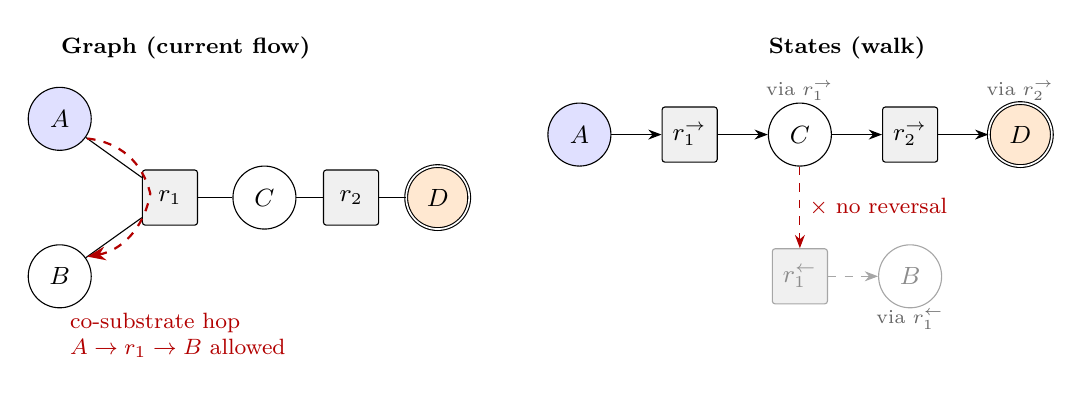
\begin{tikzpicture}[
  >=Stealth,
  met/.style={circle,draw,minimum size=8mm,inner sep=0pt},
  rxn/.style={rectangle,draw,rounded corners=1pt,minimum size=7mm,inner sep=0pt,fill=black!6},
  dim/.style={draw=black!35,text=black!45},
  every node/.style={font=\small}]
  % left: the graph
  \node[font=\footnotesize\bfseries] at (1.6,1.9) {Graph (current flow)};
  \node[met,fill=blue!12] (A) at (0,1) {$A$};
  \node[met] (B) at (0,-1) {$B$};
  \node[rxn] (r1) at (1.4,0) {$r_1$};
  \node[met] (C) at (2.6,0) {$C$};
  \node[rxn] (r2) at (3.7,0) {$r_2$};
  \node[met,fill=orange!18,double] (D) at (4.8,0) {$D$};
  \draw (A)--(r1); \draw (B)--(r1); \draw (r1)--(C); \draw (C)--(r2); \draw (r2)--(D);
  \draw[->,red!70!black,dashed,thick] (0.35,0.75) to[bend left=35] (1.15,0.05) to[bend left=35] (0.35,-0.75);
  \node[red!70!black,font=\footnotesize,align=left] at (1.5,-1.75) {co-substrate hop\\ $A\to r_1\to B$ allowed};
  % right: the states
  \begin{scope}[xshift=6.6cm]
  \node[font=\footnotesize\bfseries] at (3.4,1.9) {States (walk)};
  \node[met,fill=blue!12] (sA) at (0,0.8) {$A$};
  \node[rxn] (f1) at (1.4,0.8) {$r_1^{\fwd}$};
  \node[met] (aC) at (2.8,0.8) {$C$};
  \node[rxn] (f2) at (4.2,0.8) {$r_2^{\fwd}$};
  \node[met,fill=orange!18,double] (aD) at (5.6,0.8) {$D$};
  \node[rxn,dim] (b1) at (2.8,-1.0) {$r_1^{\bwd}$};
  \node[met,dim] (aB) at (4.2,-1.0) {$B$};
  \draw[->] (sA)--(f1); \draw[->] (f1)--(aC); \draw[->] (aC)--(f2); \draw[->] (f2)--(aD);
  \draw[->,red!70!black,dashed] (aC)--(b1) node[midway,right,font=\footnotesize] {$\times$ no reversal};
  \draw[->,black!35,dashed] (b1)--(aB);
  \node[font=\scriptsize,black!60] at (2.8,1.35) {via $r_1^{\fwd}$};
  \node[font=\scriptsize,black!60] at (5.6,1.35) {via $r_2^{\fwd}$};
  \node[font=\scriptsize,black!60] at (4.2,-1.55) {via $r_1^{\bwd}$};
  \end{scope}
\end{tikzpicture}
\caption{Toy network $r_1: A+B\rightleftharpoons C$ (reversible), $r_2: C\to D$;
source $A$, target $D$. Left: on the undirected graph, current from $A$ can leave
$r_1$ through its co-substrate $B$. Right: in the walk's state space, a walker from
$A$ goes $r_1^{\fwd}\to C\to r_2^{\fwd}\to D$. Returning through $r_1^{\bwd}$ to $B$ is
forbidden because $r_1^{\bwd}$ is the opposite of the step just taken.}
\label{fig:states}
\end{figure}

%======================================================================
\section{Absorption, leaks and the transition matrix}
%======================================================================

\paragraph{Absorption (where the DAA enters, hook 2).} Only \emph{arrival} states of
targets absorb: a walker must reach a target through a reaction. For an arrival state
$\alpha=(t\mid d)$ with $t\in\Tset$,
\begin{equation}
  a_\alpha =
  \begin{cases}
    1 & \text{full absorption (default)},\\
    1-e^{-\kappa\varphi_t} & \text{partial absorption, } \kappa \text{ given}.
  \end{cases}
  \label{eq:absorb}
\end{equation}
All other states have $a_u=0$. With partial absorption a deep drop catches almost
every walker, while a mild one lets some walk on to targets further along.

\paragraph{Transitions.} From state $u$ with out-degree $\deg^{+}(u)$ in $\X$, a
walker that is not absorbed moves along one of its arcs uniformly at random:
\begin{equation}
  Q_{uv} = \frac{1-a_u}{\deg^{+}(u)} \quad\text{for each arc } u\to v .
  \label{eq:Q}
\end{equation}

\paragraph{Leaks.} A state with no way out (a dead end) loses its walkers. More
generally, let $\X_{\mathrm{live}}$ be the states from which some absorbing state is
reachable (reverse breadth-first search, \code{\_can\_reach}). Only arcs between live
states are kept in $Q$, but $\deg^{+}(u)$ still counts \emph{all} arcs, so probability
mass that steps into a dead region is lost. Pruning dead states does not change any
result below, because a walk that enters them can never be absorbed.

%======================================================================
\section{Absorption probabilities and expected visits}
%======================================================================

Restrict everything to $\X_{\mathrm{live}}$ and let $I$ be the identity there.

\paragraph{Probability of reaching a target.} Let $h(u)$ be the probability that a
walk from state $u$ is eventually absorbed. First-step analysis gives
$h = a + Qh$, so
\begin{equation}
  (I-Q)\,h = a .
  \label{eq:h}
\end{equation}
For a source $s$, $h(s)$ is its \emph{reach probability}. Sources with $h(s)=0$ are
excluded (``no directed path to a target'').

\paragraph{Expected visits.} The fundamental matrix $N=(I-Q)^{-1}$ has $N_{su}$ =
expected number of visits to $u$ by a walk started at $s$. Its row for $s$ is
\begin{equation}
  n_s = (I-Q)^{-\top} e_s .
  \label{eq:visits}
\end{equation}
Both \eqref{eq:h} and \eqref{eq:visits} use the same LU factorisation of $I-Q$:
\eqref{eq:visits} is a transposed solve.

%======================================================================
\section{Conditioning on success: Doob's \texorpdfstring{$h$}{h}-transform}
%======================================================================

Most released walkers never reach a target: in the example run only about $20\%$ do,
the rest end in directed dead ends. Scoring all walkers would reward reactions that
lead into dead ends. The walk therefore scores only the walks that are absorbed.

\begin{proposition}
Conditioned on absorption, the walk is again a Markov chain, with transitions
$\widehat Q_{uv} = Q_{uv}\,h(v)/h(u)$ (Doob's $h$-transform). For a walk from source
$s$, the expected number of conditioned crossings of arc $u\to v$ is
\begin{equation}
  c_s(u\to v) = \frac{n_s(u)\,Q_{uv}\,h(v)}{h(s)} ,
  \label{eq:traffic}
\end{equation}
and the probability that a successful walk from $s$ ends at target $t$ is
\begin{equation}
  p_s(t) = \frac{1}{h(s)} \sum_{\alpha=(t\mid d)} n_s(\alpha)\,a_\alpha .
  \label{eq:share}
\end{equation}
\end{proposition}
\begin{proof}[Sketch]
The expected number of visits to $u$ by successful walks is $n_s(u)h(u)/h(s)$ (visit
$u$, then succeed from $u$; divide by the success probability). Multiplying by
$\widehat Q_{uv}$ gives \eqref{eq:traffic}. Equation \eqref{eq:share} counts
absorptions at $t$'s arrival states among successful walks.
\end{proof}
Under conditioning, each source sends exactly one unit of flow to the targets:
$\sum_t p_s(t)=1$. This puts the walk on the same footing as one unit of current in
current flow.

%======================================================================
\section{Folding traffic back onto the graph}
%======================================================================

\paragraph{Net edge flow.} Sum the signed arc traffic onto the edges of $G$:
\[
  F_s(e) = \sum_{\text{arcs } u\to v \text{ along } e} \operatorname{sign}(u\to v)\;c_s(u\to v),
\]
positive when, on balance, walkers move from the metabolite into the reaction.
Traffic that runs both ways along an edge cancels.

\paragraph{Throughput.} As in current flow,
\begin{equation}
  T_s(v) = \tfrac12 \sum_{e\ni v} |F_s(e)| \;-\; \tfrac12\, p_s(v)\,\mathbf 1[v\in\Tset],
  \qquad T_s(s)=0,\qquad T_s(v)\leftarrow\max\{T_s(v),0\}.
  \label{eq:throughput}
\end{equation}
A walker absorbed at a target enters but does not leave, so half of its absorbed share
is removed: a target scores only the flow it relays onwards. A source's own walkers
are not counted at that source.

\paragraph{Direction of use.} For a reaction $\rho$,
\[
  \mathrm{net\_forward}_s(\rho) = \sum_{\text{substrate edges } e \text{ of } \rho} F_s(e),
\]
positive when $\rho$ is used forward on balance and negative when used backward.

%======================================================================
\section{Combining sources into scores}
%======================================================================

\paragraph{Source weights (where the DAA enters, hook 1).} Walkers are released at
source $s$ in proportion to $\varphi_s$. The share of all \emph{successful} walkers
that came from $s$ is
\begin{equation}
  w_s = \frac{\varphi_s\,h(s)}{\sum_{s'\in\Sset}\varphi_{s'}\,h(s')} ,
  \qquad \textstyle\sum_s w_s = 1 .
  \label{eq:weights}
\end{equation}

\paragraph{Scores.} With the reached sources $\Sset^{*}=\{s: h(s)>0\}$:
\begin{align}
  \text{conductivity}\quad c(v) &= \textstyle\sum_{s\in\Sset^{*}} w_s\,T_s(v)
     \quad(\text{also reported as accumulated current}),\\
  \text{bottleneck}\quad \beta(v) &= \max_{s\in\Sset^{*}} T_s(v),\\
  \text{bottleneck fraction}\quad f_\tau(v) &= \textstyle\sum_{s} w_s\,\mathbf 1[T_s(v)\ge\tau],\quad\tau=0.5,\\
  \text{edge traffic}\quad \bar F_e &= \textstyle\sum_s w_s |F_s(e)|,\qquad F^{\max}_e=\max_s|F_s(e)|,\\
  \text{net forward}\quad \mathrm{nf}(\rho) &= \textstyle\sum_s w_s\,\mathrm{net\_forward}_s(\rho).
\end{align}
Leave-one-out scores are not defined for the walk; those columns are empty and
\code{--scoring loo} is refused.

\paragraph{Reported per metabolite and per run.} For a source, the
\code{eff\_conductance} field holds its reach probability $h(s)$; for a target, its
share of successful walkers $\sum_s w_s p_s(t)$. A pair $(s,t)$ is ``reached'' if
$p_s(t)>0$; others are excluded (``no walk reaches this target''). The run summary
adds the success fraction $\sum_s\varphi_s h(s)/\sum_s\varphi_s$, the number of
unreached sources, and the state, live-state and arc counts.

%======================================================================
\section{One-sided data}
%======================================================================
If only sources are significant, the measured but unchanged metabolites (the ground)
absorb every walker ($a=1$ at their arrival states). If only targets are significant,
walkers start evenly from the ground ($\varphi=1$ each). Ground nodes are not scored as
endpoints.

%======================================================================
\section{From node scores to ranked genes and pathways}
%======================================================================
Identical to current flow (\code{scoring.py}): a reaction's final score is the mean
percentile rank of $c$ and $\beta$; a gene takes its best reaction; pathways are tested
by hypergeometric over-representation among the top 100 reactions with
Benjamini--Hochberg correction. \code{reactions.tsv} gains the \code{net\_forward}
column. The Cytoscape subnetwork keeps edges with $F^{\max}_e\ge0.1$.

%======================================================================
\section{Computation}
%======================================================================
\begin{enumerate}[nosep]
  \item Build $\X$ and its arcs once ($21{,}787$ states on Human-GEM).
  \item Reverse BFS from absorbing states; keep live states ($16{,}951$ in the example run).
  \item One sparse LU of $I-Q$ (\code{scipy.sparse.linalg.splu}), about $0.3$\,s.
  \item Solve \eqref{eq:h} once; solve \eqref{eq:visits} for blocks of 128 sources.
  \item Sparse products fold traffic onto edges and nodes.
\end{enumerate}
That is $1+|\Sset|$ solves, against $|\Sset|+|\Tset|$ for current flow.

%======================================================================
\section{Properties and limits}
%======================================================================
\begin{itemize}
  \item \textbf{Respects direction.} Irreversible reactions are used only forward;
        reversible ones either way, recorded in \code{net\_forward}.
  \item \textbf{No co-substrate hops}, including the two-step hop through a
        reversible reaction.
  \item \textbf{Uses fold change} as release weights, and optionally as absorption
        strength.
  \item \textbf{Targets compete.} A walker stops at the first target that absorbs
        it, so with full absorption a target behind another target receives little.
        Partial absorption ($\kappa$) relaxes this; on the benchmark it changed
        little.
  \item \textbf{Throughput can exceed 1.} Directed cycles of irreversible reactions
        can circulate walkers before they leave.
  \item \textbf{Sensitive to direction annotations.} A reaction marked irreversible
        in the wrong direction blocks every route through it. If the measured
        metabolites point away from the block, as with shunt products, walkers cannot
        reach it.
  \item \textbf{Only successful walks count.} When few walkers reach a target (low
        success fraction), scores rest on a small share of the released walkers.
\end{itemize}

\begin{remark}[Relation to current flow and to RWR]
On an undirected graph, unit current from $s$ to $t$ equals the expected net edge
crossings of a simple random walk from $s$ absorbed at $t$ (Newman, 2005). The walk
here changes three things: it is directed (on the state space), all targets absorb
together, and sources are weighted by fold change and conditioned on success. It is
not a random walk with restart (RWR): an RWR walker returns to its seed with a fixed
probability at every step and the score is its stationary visit frequency, whereas
here walks end at a target or a dead end and the score is the traffic of successful
walks.
\end{remark}

%======================================================================
\section{Validation}
%======================================================================
\code{tests/test\_walk.py} checks the rules on hand-built networks: a chain carries
$1$; a backward-only reaction blocks the forward route and is used backward
(net forward $=-1$); no co-substrate hop, even in two steps; a dead-end branch leaks
half the walkers and scores $0$; partial absorption splits as $1-e^{-\kappa\varphi}$
predicts; $\varphi=3$ vs.\ $1$ splits conductivity $0.75/0.25$; one-sided ground
absorption. A Monte Carlo simulation (40{,}000 walkers per source) on a network with
branches, a reversible reaction, a directed cycle, a dead end and partial absorption
agrees with the exact solution (maximum difference $0.005$).

%======================================================================
\section{Benchmark}
%======================================================================
Inborn errors of metabolism: rank of the causal gene among $2{,}302$ network genes,
raw scoring, full absorption; lower is better. Source: \code{docs/decisions.md}, D17.

\begin{center}
\begin{tabular}{@{}llrr@{}}
\toprule
Level & Measure & Current flow & Absorbing walk\\
\midrule
Group (20 primary disorders) & median rank & 88.5 & 48\\
 & in top 100 & 11 & 13\\
 & in top 10 & 3 & 5\\
Patient (159 primary patients) & median rank & 134 & 67\\
 & in top 100 & 47\% & 55\%\\
 & in top 10 & 5\% & 28\%\\
\bottomrule
\end{tabular}
\end{center}

The walk ranks the causal gene better for $71\%$ of patients and in 14 of 20
disorders. Largest group-level gains: MSUD $33\to1$, PKU $186\to16$, propionic
acidaemia $1{,}187\to176$, citrullinaemia $82\to20$. Losses show where direction hurts.
In AADC deficiency ($88\to1{,}317$) the main source, 3-O-methyldopa, is made
irreversibly \emph{from} the blocked substrate L-DOPA, so walkers cannot run back to
the block. In homocystinuria ($181\to765$) the only target is cortisol, which carries
no information about the block. In both, fewer than $4\%$ of walkers reach a target.
Partial absorption barely matters (group medians $45.5$--$47$ for
$\kappa=0.5,1,2$, against $48$).

\paragraph{Status.} Not the default. It changes protocol \S2.3, the evidence is one
benchmark, and the blind predictions (D14) were made with current flow. To be decided
before the next blind round. Not yet tried: biased steps (hook 3), unchanged
metabolites as leaks (hook 4), and the reverse ``activation'' orientation.

%======================================================================
\section{Implementation map}
%======================================================================
\begin{center}
\small
\begin{tabularx}{\linewidth}{@{}lX@{}}
\toprule
Code (\code{metaboenrich/walk.py}) & What it computes\\
\midrule
\code{walk\_states(graph)} & state space $\X$, arcs, arc edges and signs\\
\code{\_can\_reach(\dots)} & live states $\X_{\mathrm{live}}$\\
\code{absorbing\_walk(\dots)}: \code{absorb}, \code{q} & $a$ \eqref{eq:absorb}, $Q$ \eqref{eq:Q}\\
\quad \code{splu}, \code{lu.solve(absorb)} & $h$ \eqref{eq:h}, weights \eqref{eq:weights}\\
\quad \code{lu.solve(E, trans="T")} & visits $n_s$ \eqref{eq:visits}\\
\quad \code{C}, \code{absorbed} & traffic \eqref{eq:traffic}, target shares \eqref{eq:share}\\
\quad \code{M @ C}, \code{absB\_T}, \code{S\_fwd} & $F_s$, throughput \eqref{eq:throughput}, net forward\\
\code{FlowResult}, \code{walk\_info} & same container as current flow, plus run numbers\\
\bottomrule
\end{tabularx}
\end{center}
\noindent Command line and benchmark:
\begin{quote}\small
\code{python -m metaboenrich --daa \dots{} --mode walk [--walk-kappa K]}\\
\code{python -m metaboenrich.benchmark --method walk [--walk-kappa K]}
\end{quote}

\section*{References}
\begin{itemize}[nosep,leftmargin=*]
  \item Doob, J.\,L. (1957). Conditional Brownian motion and the boundary limits of
        harmonic functions. \emph{Bull.\ Soc.\ Math.\ France} 85, 431--458.
  \item Kemeny, J.\,G.\ and Snell, J.\,L. (1960). \emph{Finite Markov Chains}.
        Van Nostrand (absorbing chains, fundamental matrix).
  \item Newman, M.\,E.\,J. (2005). A measure of betweenness centrality based on random
        walks. \emph{Social Networks} 27, 39--54.
  \item Doyle, P.\,G.\ and Snell, J.\,L. (1984). \emph{Random Walks and Electric
        Networks}. Mathematical Association of America.
  \item Metaboenrich \code{docs/decisions.md}, D17.
\end{itemize}

\end{document}
